\documentclass[11pt]{article}
\usepackage{url}
\usepackage{color,rotating,epic,subfigure,amssymb,cite,amscd,amsmath,multirow,bm,url,rotating}
\usepackage[margin=2cm]{geometry}
\usepackage{authblk}

\usepackage{graphicx,epstopdf}
\usepackage{multirow,threeparttable, makecell}
\usepackage{amssymb, siunitx}
\usepackage{amsthm}
\usepackage{epsfig}
\usepackage{cite}
\usepackage{verbatim}
\usepackage{tikz}
\usepackage{longtable}
%\usepackage{gantt}
\usetikzlibrary{arrows,decorations.pathmorphing,backgrounds,fit,positioning,shapes.symbols,chains}
\usetikzlibrary{positioning}
\usepackage{tikz-qtree}
\usepackage{caption}
%\usepackage[format=plain,
%            labelfont={bf,it},
%            textfont=it]{caption}

%\renewcommand{\tableshortname}{Supplementary Table}
\newcommand{\beginsupplement}{%
        \setcounter{table}{1}
        \setcounter{figure}{0}
        \renewcommand{\thefigure}{Supplementary \arabic{figure}}%
     }
     

\begin{document}
\title{\textbf{Prioritization of Exome Data by Image Analysis \\ Supplementary Material}}
\author[1, 2]{Hsieh, Tzung-Chien \textsuperscript{*}}
\author[2, 3]{Mensah, Martin-Atta \textsuperscript{*}}
\author[2, 3]{Pantel, Jean Tori}
\author[]{PEDIA consortium}
\author[1]{Krawitz, Peter}
\affil[1]{\footnotesize Institute of Genomic Statistics and Bioinformatics, 
  University of Bonn, Bonn, Germany}
\affil[2]{\footnotesize Charité –Universitätsmedizin Berlin, corporate
  member of Freie Universität Berlin, Humboldt-Universität zu Berlin,
  and Berlin Institute of Health, Institute of Medical Genetics and
  Human Genetics, Berlin, Germany }
\affil[3]{\footnotesize Berlin Institute ofHealth (BIH), Anna-Louisa-Karsch 2, 10178
  Berlin, German}
\date{}
\maketitle
\clearpage

\beginsupplement
The influence of the ethnic background on the performance of the PEDIA approach was analyzed by spiking in the disease-causing mutations into the different populations of the 1000 genomes project (ACB, African Caribbeans in Barbados; ASW Americans of African Ancestry in SW USA; BEB, Bengali from Bangladesh; CDX, Chinese Dai in Xishuangbanna, China; CEU Western European Ancestry; CHBHan Chinese in Beijing, China; CHS, Southern Han Chinese; CLM, Colombians from Medellin, Colombia; ESN, Esan in Nigeria; FIN, Finnish in Finland; GBR, British in England Scotland; GIH, Gujarati Indian from Houston Texas; GWD, Gambian in Western Divisions in the Gambia; IBS, Iberian Population in Spain; ITU, Indian Telugu from the UK; JPT, Japanese in Tokyo, Japan; KHV, Kinh in Ho Chi Minh City, Vietnam; LWK, Luhya in Webuye, Kenya; MSL, Mende in Sierra Leone; MXL, Mexican Ancestry from Los Angeles USA; PEL, Peruvians from lima, Peru; PJL, Punjabi from Lahore, Pakistan; PUR, Puerto Ricans from Puerto Rico; STU, Sri Lankan Tamil from the UK; TSI, Toscani in Italia; YRI, Yoruba in Ibadan, Nigeria).

\begin{figure}[ht]
  \begin{center}
    \graphicspath{{./figures/}}
    \begin{tabular}{c}
      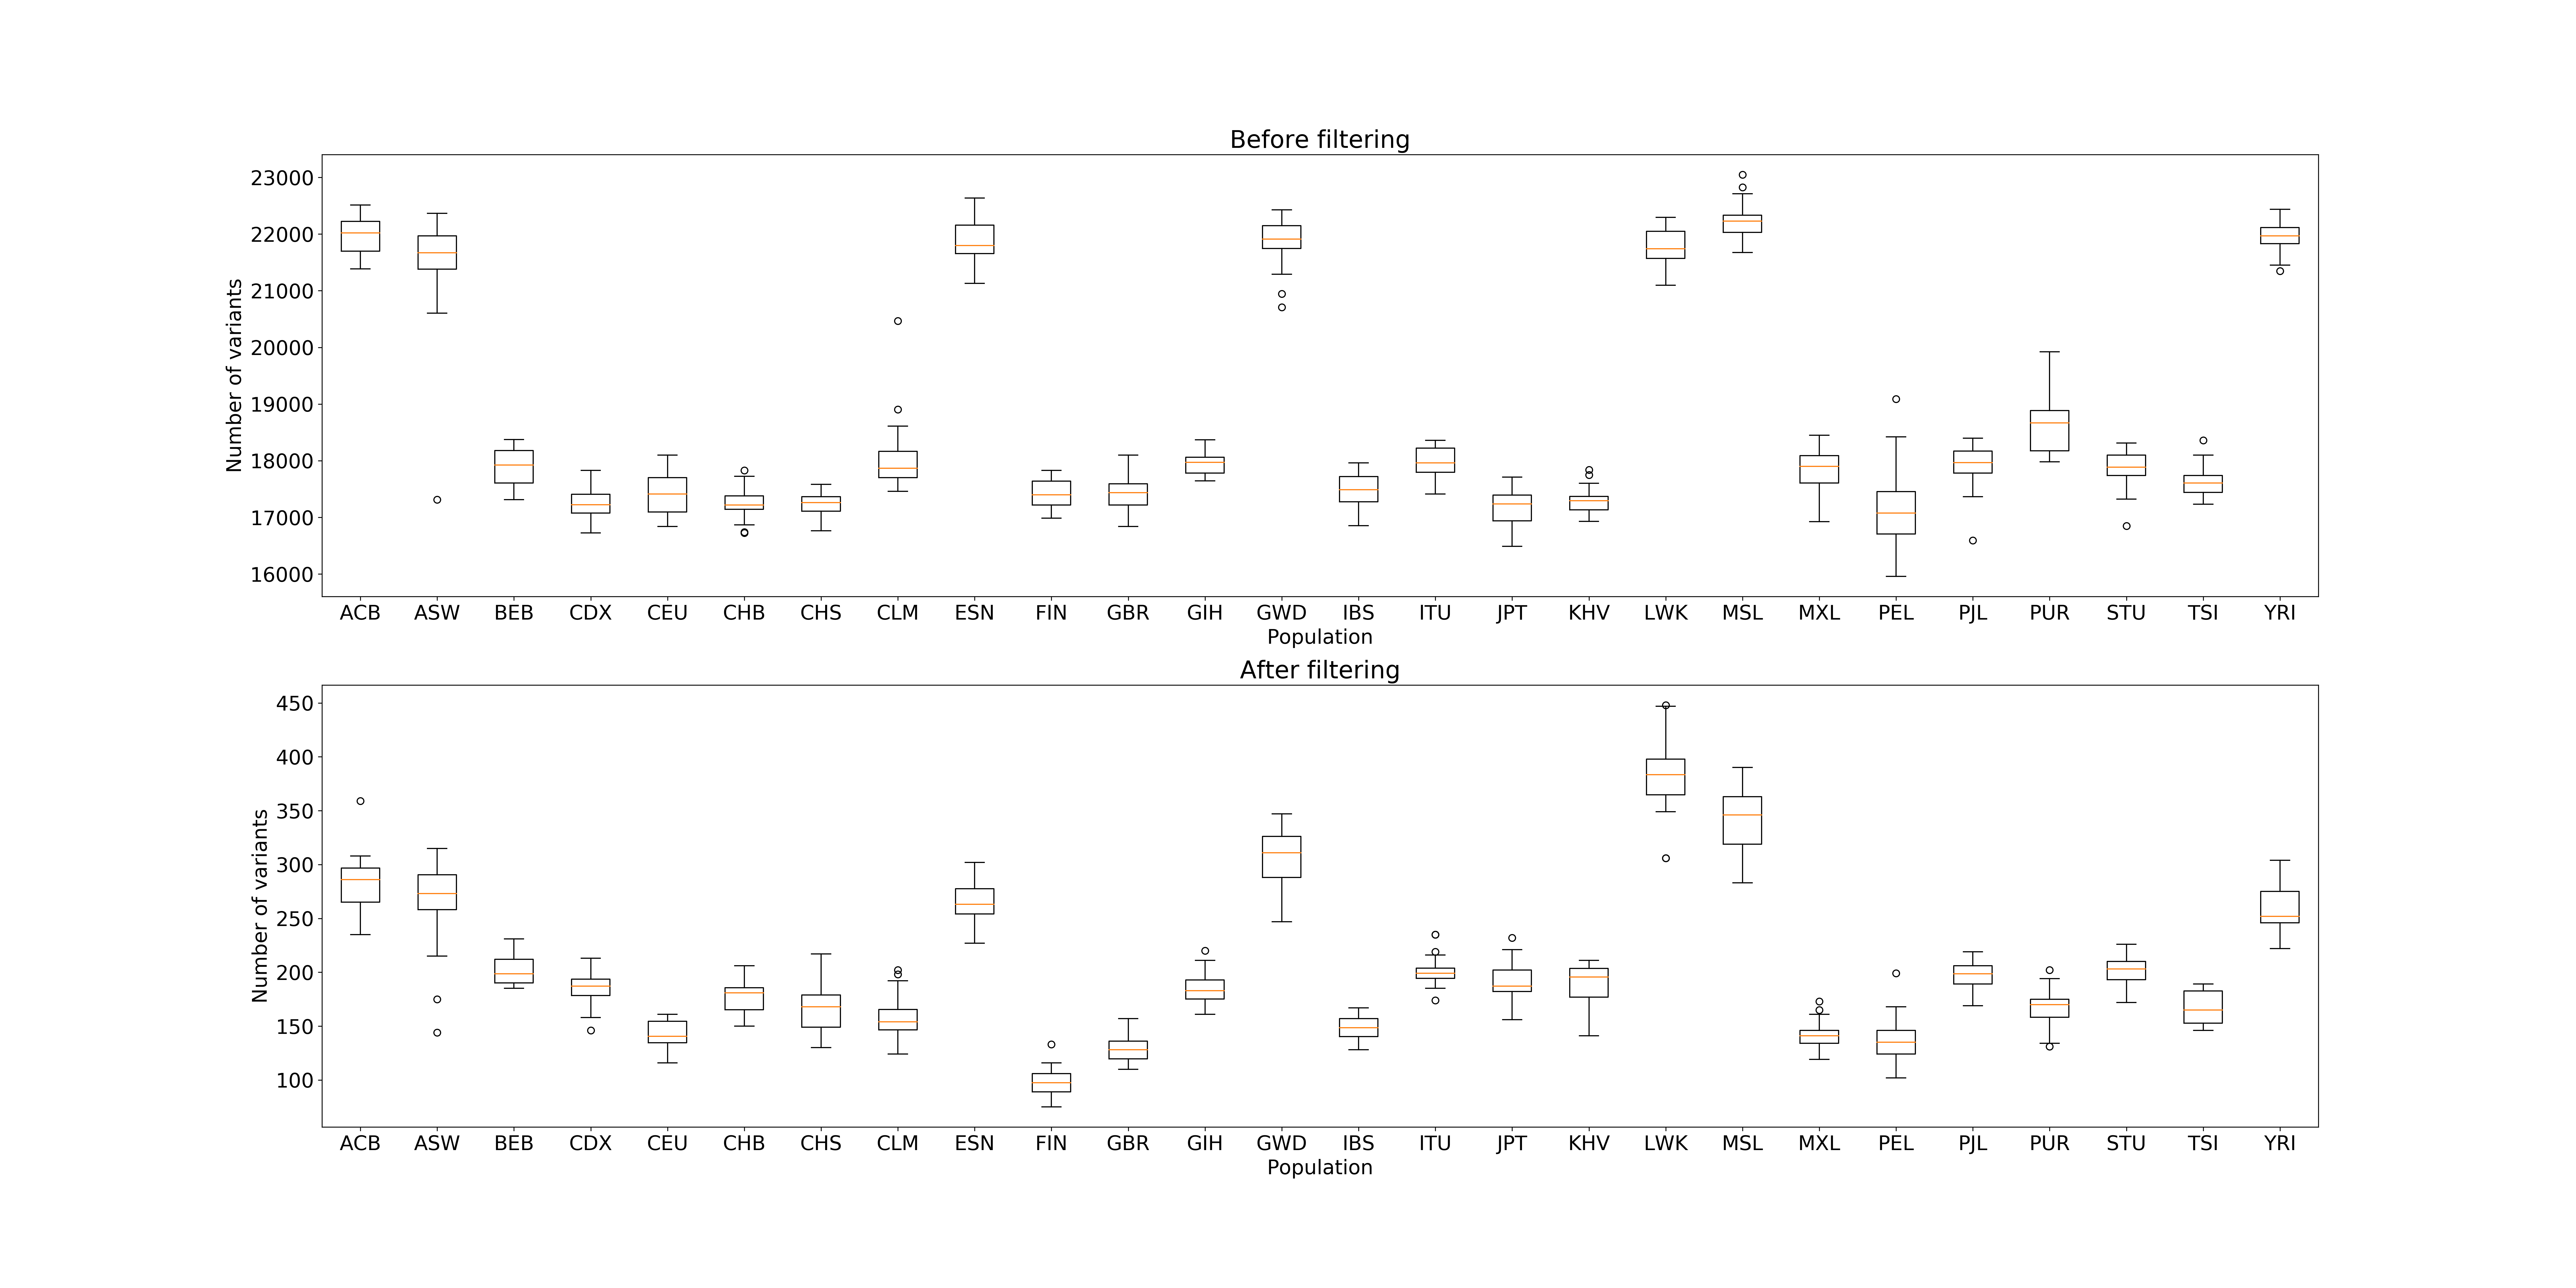
\includegraphics[width=18 cm, height= 9 cm]{population_variants_num.png}
    \end{tabular}
  \caption*{\textbf{Supplementary Figure 1:} The number of variants that are called in reference-guided exome sequencing varies depending on the ethnic background. Filtering according to Wright, et al., results in 100 to 400 rare variants, with the smallest numbers observed in individuals from Finland and the largest in individuals from Kenya.}
  \end{center}
\end{figure}

\begin{figure}[ht]
  \begin{center}
    \graphicspath{{./figures/}}
    \begin{tabular}{c}
      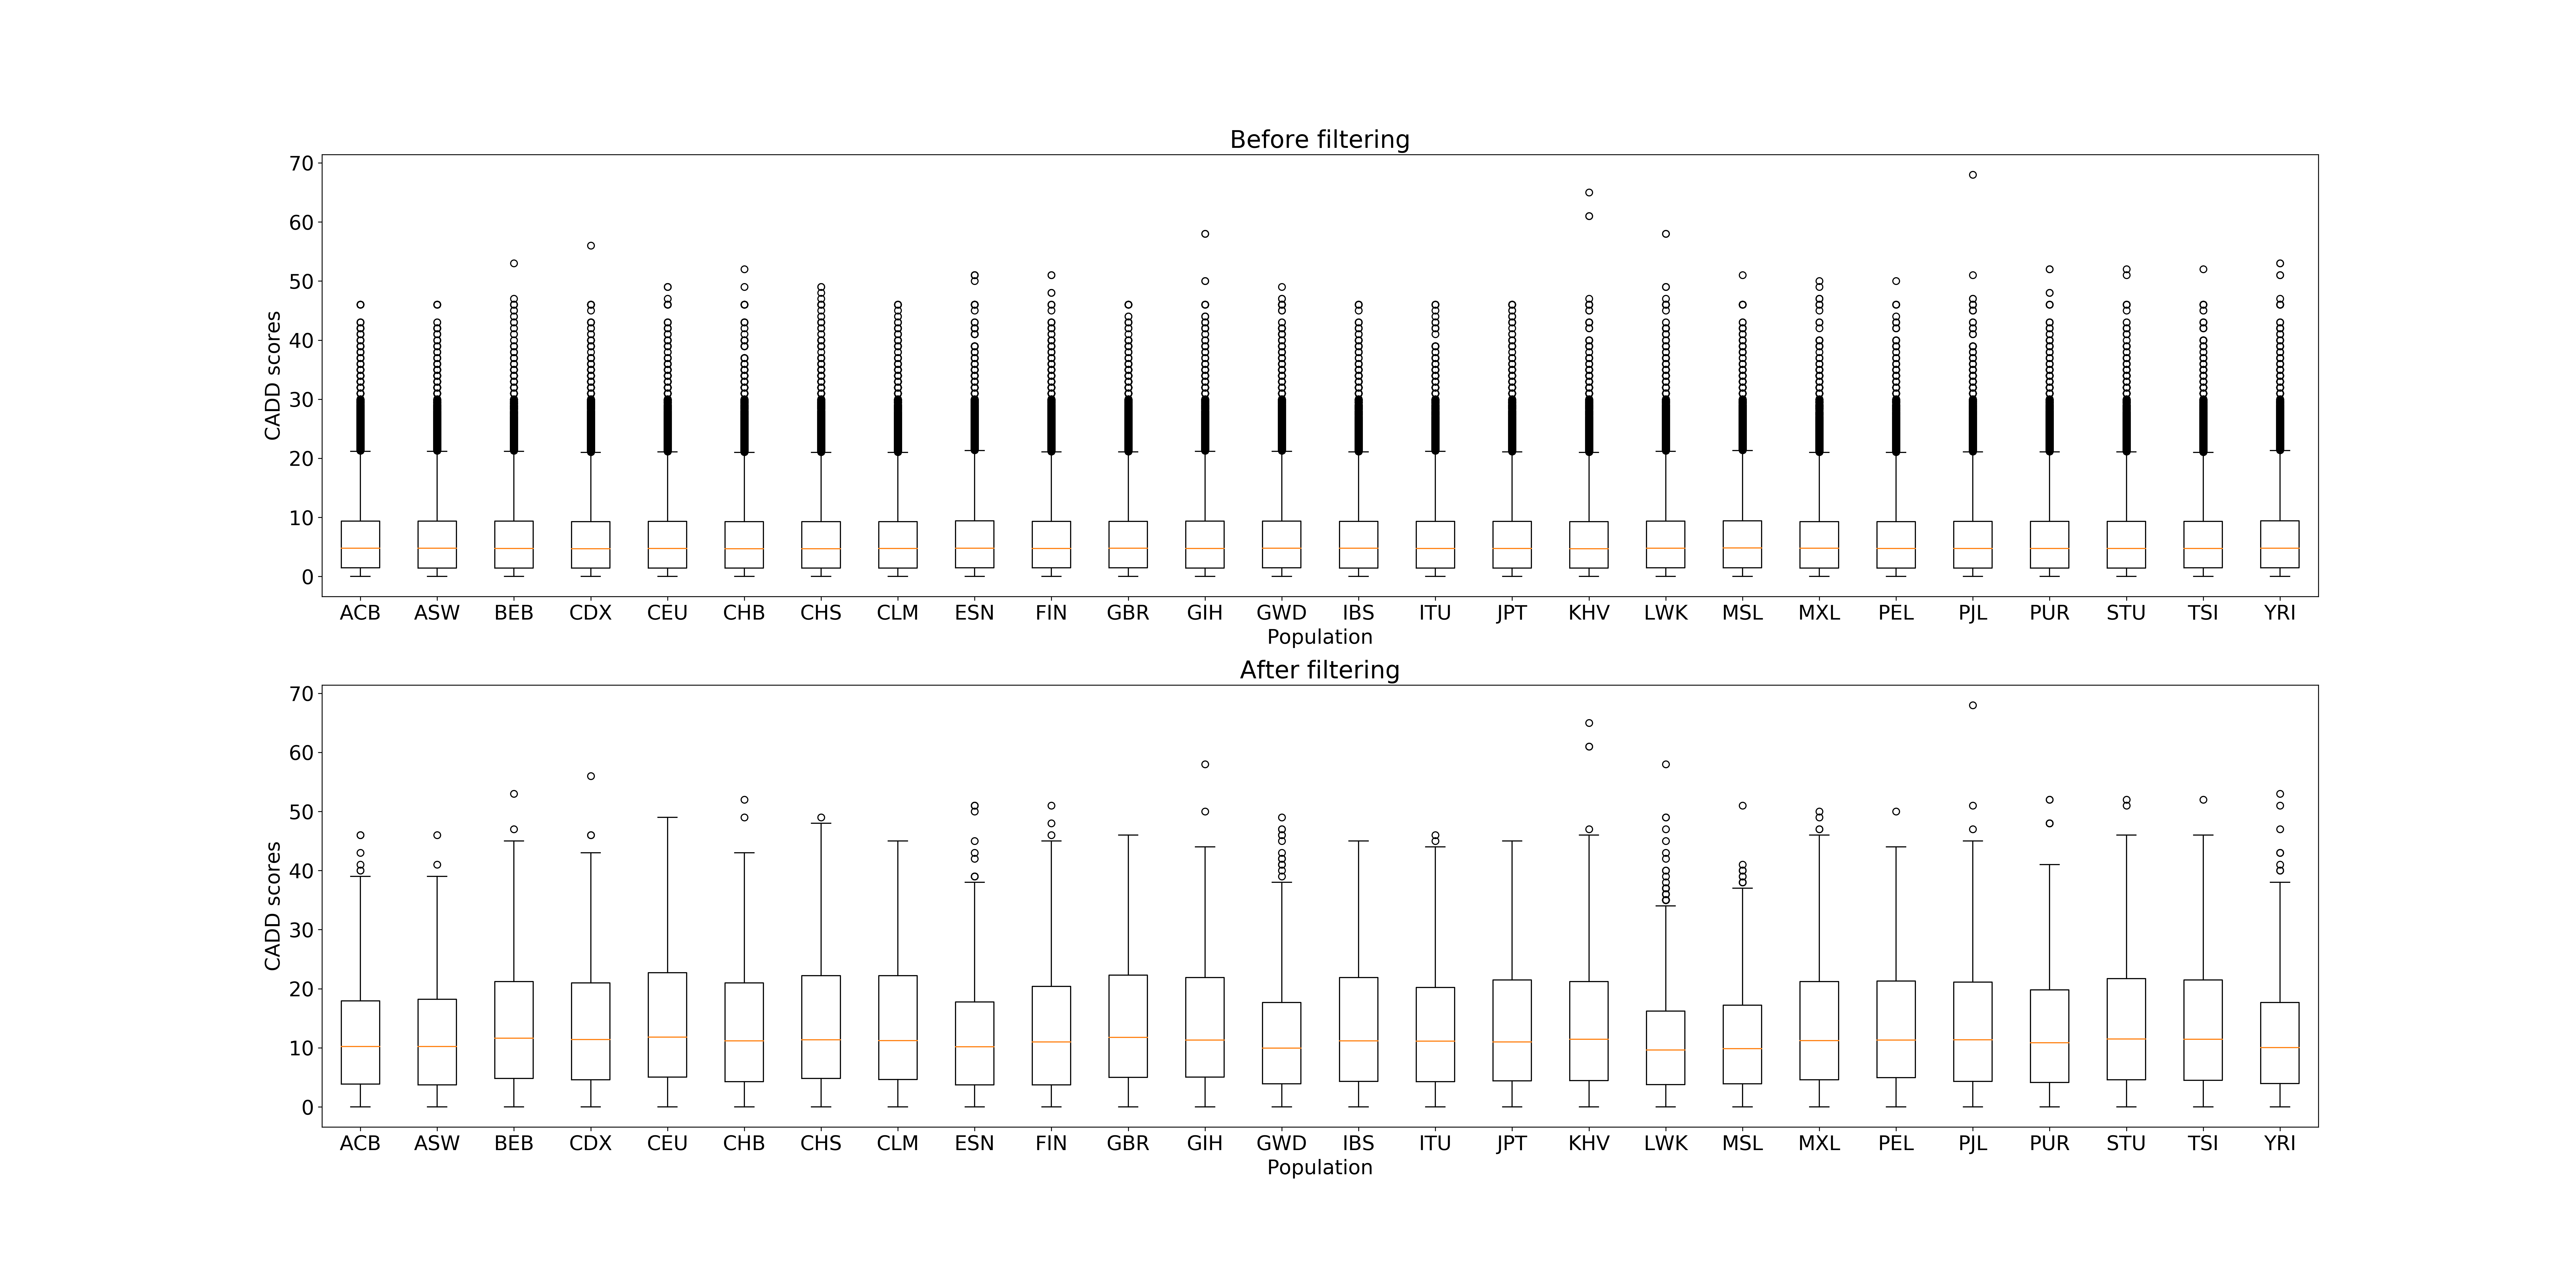
\includegraphics[width=18 cm, height= 9 cm]{population_cadd.png}
    \end{tabular}
  \caption*{\textbf{Supplementary Figure 2:} The distribution of CADD scores is less dependent on the ethnic background. In all populations there is a shift in the median of the CADD scores after filtering for rare variants.}
  \end{center}
\end{figure}

\begin{figure}[ht]
  \begin{center}
    \graphicspath{{./figures/}}
    \begin{tabular}{c}
      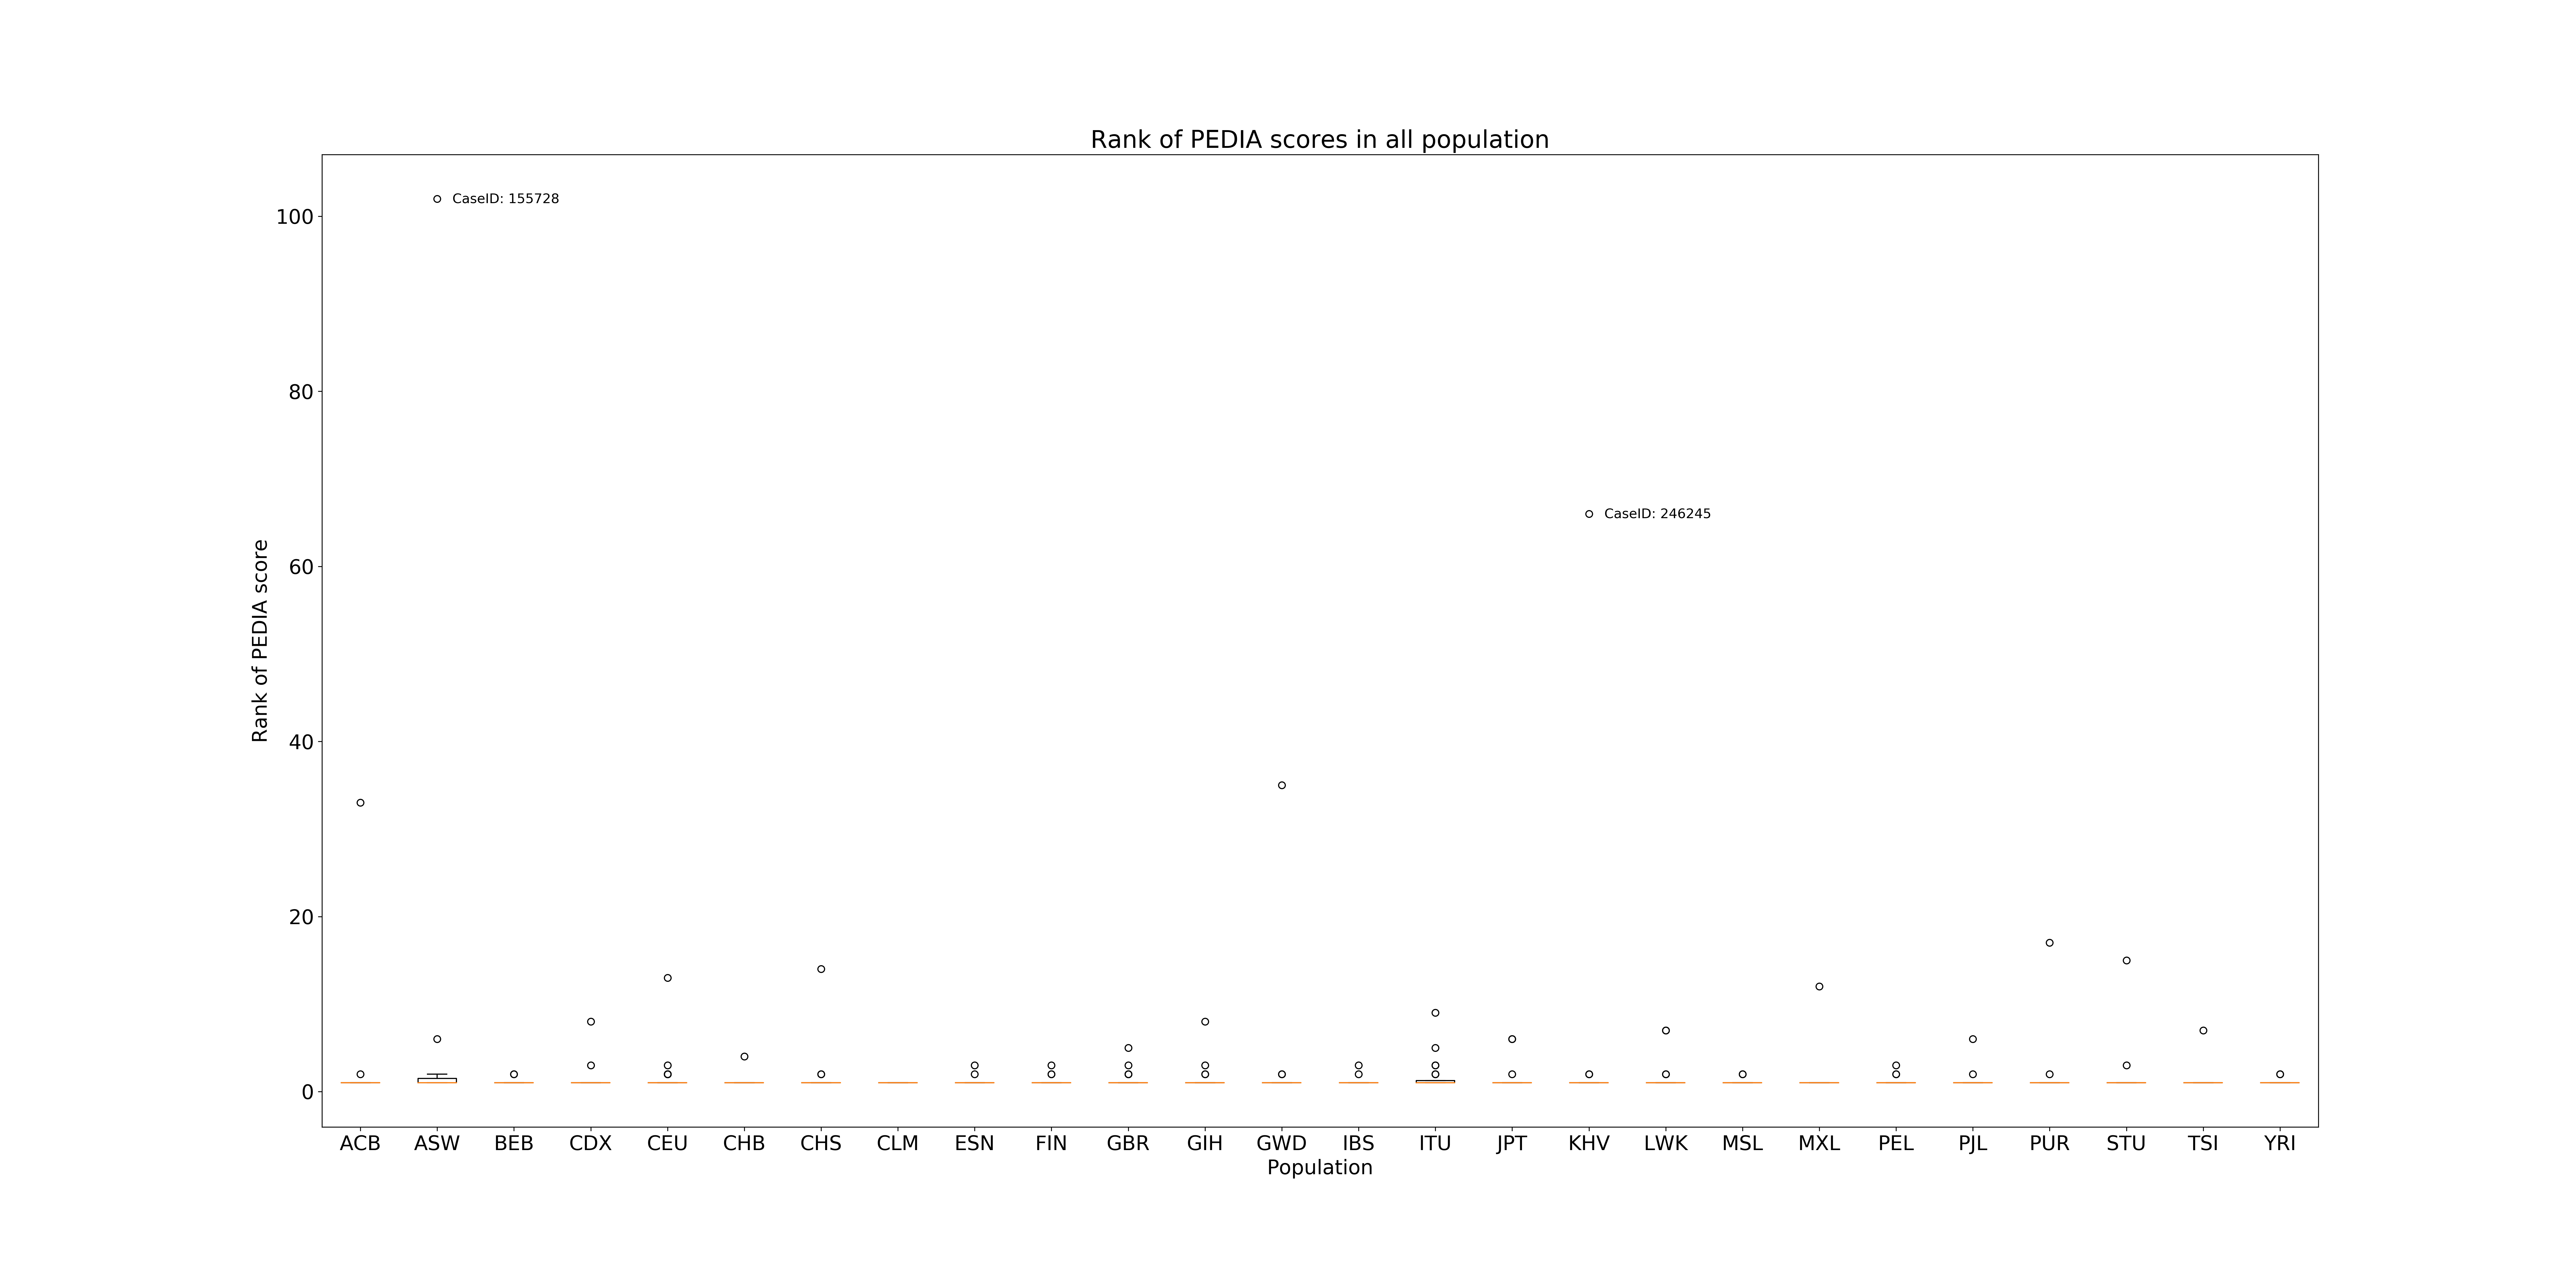
\includegraphics[width=18 cm, height= 9 cm]{population_rank.png}
    \end{tabular}
  \caption*{\textbf{Supplementary Figure 3:} The disease-causing
mutations of the PEDIA cohort have been spiked into randomly selected
samples from the 1KGP project. Shown are the results of one such
simulation. The mean rank that the disease-causing gene achieves, does
not depend on the ethnic background. The phenotypic and molecular data
of poorly performing examples, e.g. cases 155728 and 246245 (see
Supplementary Table 1 for details) yield lowest ranks in all population.}
  \end{center}
\end{figure}
\begin{center}
\begin{table}[ht]
\caption*{\textbf{Supplementary Table 2:} Comparision results of using
different scores for gene prioritization. First column indicates the
scores used in each row. The second and third columns are the Top-1 and
Top-10 accuracy and confidance interval. For genes with the same PEDIA
score, the highest (worst) rank was used for all of them, as this
represents best the associated time for the workup. (F, Feature match score. C, CADD score. G, Gestalt score. P, Phenomizer score. B, Boqa score).}\medskip
\label{result}
\centering
\begin{tabular}{|c|c|c|} \hline
&Top-1 (\%)&Top-10 (\%)\\ \hline 
\multicolumn{3}{|c|}{\textbf{Photo + Exome + Feature}}\\ \hline 
F,C,G,B,P&89.4 \small{[81.4 - 97.4]} & 98.7 \small{[95.7 - 100]}\\ \hline 
C,G,B,P&89.0 \small{[80.0 - 98.0]} & 98.7 \small{[95.1 - 100]}\\ \hline 
F,C,G,P&89.1 \small{[79.9 - 98.3]} & 98.5 \small{[95.1 - 100]}\\ \hline 
F,C,G,B&87.9 \small{[78.7 - 97.1]} & 98.1 \small{[94.7 - 100]}\\ \hline 
C,G,P&88.5 \small{[79.3 - 97.7]} & 98.2 \small{[93.8 - 100]}\\ \hline 
C,G,B&86.0 \small{[75.4 - 96.6]} & 97.8 \small{[95.8 - 99.8]}\\ \hline 
F,C,G&87.8 \small{[76.4 - 99.2]} & 97.9 \small{[94.1 - 100]}\\ \hline 
\multicolumn{3}{|c|}{\textbf{Photo + Exome}}\\ \hline 
C,G&82.6 \small{[67.6 - 97.6]} & 97.5 \small{[95.1 - 99.9]}\\ \hline 
\multicolumn{3}{|c|}{\textbf{Photo + Feature}}\\ \hline 
F,G,B,P&25.1 \small{[1.7 - 48.5]} & 69.2 \small{[35.8 - 100]}\\ \hline 
G,B,P&24.0 \small{[3.0 - 45.0]} & 65.0 \small{[32.4 - 97.6]}\\ \hline 
F,G,P&20.5 \small{[1.7 - 39.3]} & 67.2 \small{[33.0 - 100]}\\ \hline 
F,G,B&23.1 \small{[1.5 - 44.7]} & 65.9 \small{[36.1 - 95.7]}\\ \hline 
G,P&18.6 \small{[2.6 - 34.6]} & 61.3 \small{[24.9 - 97.7]}\\ \hline 
G,B&22.0 \small{[4.6 - 39.4]} & 58.6 \small{[31.4 - 85.8]}\\ \hline 
F,G&16.8 \small{[0 - 34.4]} & 59.2 \small{[29.8 - 88.6]}\\ \hline 
\multicolumn{3}{|c|}{\textbf{Exome + Feature}}\\ \hline 
F,C,B,P&74.4 \small{[60.0 - 88.8]} & 93.7 \small{[88.5 - 98.9]}\\ \hline 
C,B,P&61.4 \small{[43.2 - 79.6]} & 89.0 \small{[84.2 - 93.8]}\\ \hline 
F,C,P&74.1 \small{[64.1 - 84.1]} & 93.8 \small{[87.2 - 100]}\\ \hline 
F,C,B&65.8 \small{[47.8 - 83.8]} & 91.3 \small{[82.1 - 100]}\\ \hline 
C,P&57.9 \small{[39.1 - 76.7]} & 88.7 \small{[81.3 - 96.1]}\\ \hline 
C,B&35.5 \small{[12.1 - 58.9]} & 62.8 \small{[40.4 - 85.2]}\\ \hline 
F,C&65.1 \small{[49.1 - 81.1]} & 90.9 \small{[80.5 - 100]}\\ \hline 
\multicolumn{3}{|c|}{\textbf{Photo}}\\ \hline 
G&14.3 \small{[0.3 - 28.3]} & 48.6 \small{[23.4 - 73.8]}\\ \hline 
\multicolumn{3}{|c|}{\textbf{Exome}}\\ \hline 
C&14.1 \small{[0 - 31.1]} & 44.6 \small{[13.6 - 75.6]}\\ \hline 
\multicolumn{3}{|c|}{\textbf{Feature}}\\ \hline 
F,B,P&16.4 \small{[0 - 34.2]} & 54.4 \small{[25.4 - 83.4]}\\ \hline 
B,P&16.2 \small{[0.8 - 31.6]} & 48.9 \small{[21.9 - 75.9]}\\ \hline 
F,P&16.7 \small{[0 - 36.9]} & 53.8 \small{[27.0 - 80.6]}\\ \hline 
F,B&16.4 \small{[0 - 34.4]} & 53.8 \small{[24.6 - 83.0]}\\ \hline 
P&1.8 \small{[0 - 4.6]} & 16.4 \small{[0 - 33.2]}\\ \hline 
B&11.2 \small{[0 - 28.8]} & 46.4 \small{[22.0 - 70.8]}\\ \hline 
F&13.4 \small{[0 - 29.4]} & 50.7 \small{[25.5 - 75.9]}\\ \hline 
\end{tabular}
\end{table}
\end{center}

\clearpage
\footnotesize
\begin{longtable}[ht]{|c|c|p{8.4cm}|c|c|}
\caption*{\textbf{Supplementary Table 3:} Comparision of results by using DeepGestalt and PEDIA on DeepGestalt publication test set. The PEDIA rank is the average rank.}\\  \hline
Index&Syndrome Name&\makecell{Photo Link}&DeepGestalt&PEDIA\\ \hline 
1&\makecell{Alagille Syndrome}&https://app.face2gene.com/dg/lmd/110/photo/345&28&1.9\\ \hline 
2&\makecell{Nijmegen Breakage \\Syndrome; NBS}&https://app.face2gene.com/dg/lmd/347/photo/4734&2&1.0\\ \hline 
3&\makecell{Nijmegen Breakage \\Syndrome; NBS}&https://app.face2gene.com/dg/lmd/347/photo/4730&2&1.0\\ \hline 
4&\makecell{Craniodiaphyseal \\Dysplasia; CDD}&https://app.face2gene.com/dg/lmd/373/photo/1088&1&1.0\\ \hline 
5&\makecell{Noonan Syndrome}&https://app.face2gene.com/dg/lmd/1946/photo/5976&19&1.4\\ \hline 
6&\makecell{Noonan Syndrome}&https://app.face2gene.com/dg/lmd/1946/photo/5985&11&1.1\\ \hline 
7&\makecell{Smith-Lemli-Opitz \\Syndrome; SLOS}&https://app.face2gene.com/dg/lmd/1608/photo/4893&1&1.0\\ \hline 
8&\makecell{Kabuki Syndrome}&https://app.face2gene.com/dg/lmd/893/photo/2567&1&1.0\\ \hline 
9&\makecell{Focal Facial Dermal \\Dysplasia 3, Setleis \\Type; FFDD3}&https://app.face2gene.com/dg/lmd/1570/photo/4760&5&1.0\\ \hline 
10&\makecell{Burn-Mckeown \\Syndrome; BMKS}&https://app.face2gene.com/dg/lmd/2907/photo/6717&1&1.0\\ \hline 
11&\makecell{Burn-Mckeown \\Syndrome; BMKS}&https://app.face2gene.com/dg/lmd/2907/photo/6716&1&1.0\\ \hline 
12&\makecell{Burn-Mckeown \\Syndrome; BMKS}&https://app.face2gene.com/dg/lmd/2907/photo/6719&18&2.8\\ \hline 
13&\makecell{Burn-Mckeown \\Syndrome; BMKS}&https://app.face2gene.com/dg/lmd/2907/photo/6720&1&1.2\\ \hline 
14&\makecell{Meier-Gorlin Syndrome \\1; MGORS1}&https://app.face2gene.com/dg/lmd/808/photo/2269&30&1.2\\ \hline 
16&\makecell{Trichorhinophalangeal \\Syndrome, Type II; \\TRPS2}&https://app.face2gene.com/dg/lmd/971/photo/2778&1&1.0\\ \hline 
17&\makecell{Acrocallosal Syndrome; \\ACLS}&https://app.face2gene.com/dg/lmd/23/photo/80&7&1.6\\ \hline 
18&\makecell{Cohen Syndrome; \\COH1}&https://app.face2gene.com/dg/lmd/333/photo/1003&1&1.0\\ \hline 
19&\makecell{Schwartz-Jampel \\Syndrome, Type 1; SJS1}&https://app.face2gene.com/dg/lmd/1548/photo/4685&9&1.1\\ \hline 
20&\makecell{Treacher Collins \\Syndrome 1; TCS1}&https://app.face2gene.com/dg/lmd/1720/photo/5245&1&1.0\\ \hline 
21&\makecell{Trichorhinophalangeal \\Syndrome}&https://app.face2gene.com/dg/lmd/1730/photo/5290&1&1.0\\ \hline 
22&\makecell{Velocardiofacial \\Syndrome}&https://app.face2gene.com/dg/lmd/1762/photo/8285&3&1.0\\ \hline 
23&\makecell{Smith-Lemli-Opitz \\Syndrome; SLOS}&https://app.face2gene.com/dg/lmd/1608/photo/8342&1&1.0\\ \hline 
24&\makecell{Marfan Syndrome; MFS}&https://app.face2gene.com/dg/lmd/1057/photo/8255&1&1.0\\ \hline 
26&\makecell{Mowat-Wilson Syndrome; \\MOWS}&https://app.face2gene.com/dg/lmd/4211/photo/13183&1&1.0\\ \hline 
27&\makecell{Mowat-Wilson Syndrome; \\MOWS}&https://app.face2gene.com/dg/lmd/4211/photo/13743&1&1.0\\ \hline 
28&\makecell{Mowat-Wilson Syndrome; \\MOWS}&https://app.face2gene.com/dg/lmd/4211/photo/13744&1&1.0\\ \hline 
29&\makecell{3MC Syndrome 3; \\3MC3}&https://app.face2gene.com/dg/lmd/1048/photo/14730&2&1.0\\ \hline 
30&\makecell{Sotos Syndrome 2; \\SOTOS2}&https://app.face2gene.com/dg/lmd/1617/photo/15149&1&1.1\\ \hline 
31&\makecell{Sotos Syndrome 2; \\SOTOS2}&https://app.face2gene.com/dg/lmd/1617/photo/15152&1&1.0\\ \hline 
32&\makecell{Treacher Collins \\Syndrome 1; TCS1}&https://app.face2gene.com/dg/lmd/1720/photo/5227&1&1.0\\ \hline 
33&\makecell{Coffin-Lowry Syndrome; \\CLS}&https://app.face2gene.com/dg/lmd/328/photo/958&1&1.0\\ \hline 
35&\makecell{Mowat-Wilson Syndrome; \\MOWS}&https://app.face2gene.com/dg/lmd/4211/photo/16768&1&1.0\\ \hline 
36&\makecell{Donnai-Barrow \\Syndrome}&https://app.face2gene.com/dg/lmd/3473/photo/16950&49&1.2\\ \hline 
37&\makecell{Floating-Harbor \\Syndrome; FLHS}&https://app.face2gene.com/dg/lmd/596/photo/17148&17&1.3\\ \hline 
38&\makecell{Pitt-Hopkins \\Syndrome; PTHS}&https://app.face2gene.com/dg/lmd/8892/photo/17151&1&1.0\\ \hline 
39&\makecell{Marshall-Smith \\Syndrome; MRSHSS}&https://app.face2gene.com/dg/lmd/7513/photo/17204&1&1.0\\ \hline 
40&\makecell{3MC Syndrome 3; 3MC3}&https://app.face2gene.com/dg/lmd/1048/photo/17445&110&1.7\\ \hline 
42&\makecell{Waardenburg Syndrome, \\Type 1; WS1}&https://app.face2gene.com/dg/lmd/1781/photo/5438&37&1.0\\ \hline 
44&\makecell{Sotos Syndrome 2; \\SOTOS2}&https://app.face2gene.com/dg/lmd/1617/photo/4945&1&1.0\\ \hline 
45&\makecell{Pitt-Hopkins Syndrome; \\PTHS}&https://app.face2gene.com/dg/lmd/8892/photo/17999&1&1.0\\ \hline 
46&\makecell{Kabuki Syndrome}&https://app.face2gene.com/dg/lmd/893/photo/18077&1&1.0\\ \hline 
47&\makecell{Waardenburg Syndrome, \\Type 1; WS1}&https://app.face2gene.com/dg/lmd/1781/photo/8786&1&1.0\\ \hline 
48&\makecell{Waardenburg Syndrome, \\Type 1; WS1}&https://app.face2gene.com/dg/lmd/1781/photo/8794&25&1.0\\ \hline 
49&\makecell{Smith-Magenis \\Syndrome; SMS}&https://app.face2gene.com/dg/lmd/3562/photo/9086&1&1.0\\ \hline 
51&\makecell{Seckel Syndrome}&https://app.face2gene.com/dg/lmd/739/photo/9429&2&1.0\\ \hline 
52&\makecell{Rothmund-Thomson \\Syndrome; RTS}&https://app.face2gene.com/dg/lmd/1487/photo/9782&66&1.5\\ \hline 
54&\makecell{Coffin-Siris Syndrome1; \\CSS1}&https://app.face2gene.com/dg/lmd/329/photo/18535&15&1.0\\ \hline 
55&\makecell{Bohring-Opitz Syndrome; \\BOPS}&https://app.face2gene.com/dg/lmd/4337/photo/18830&1&1.0\\ \hline 
56&\makecell{SHORT syndrome}&https://app.face2gene.com/dg/lmd/1574/photo/4787&1&1.0\\ \hline 
57&\makecell{Schwartz-Jampel \\Syndrome, Type 1; SJS1}&https://app.face2gene.com/dg/lmd/1548/photo/4686&4&1.0\\ \hline 
58&\makecell{Hajdu-Cheney Syndrome; \\HJCYS}&https://app.face2gene.com/dg/lmd/722/photo/2067&1&1.0\\ \hline 
59&\makecell{Coffin-Lowry Syndrome; \\CLS}&https://app.face2gene.com/dg/lmd/328/photo/967&1&1.0\\ \hline 
60&\makecell{Baraitser-Winter \\Syndrome 1; BRWS1}&https://app.face2gene.com/dg/lmd/149/photo/430&2&1.0\\ \hline 
61&\makecell{Beckwith-Wiedemann \\Syndrome; BWS}&https://app.face2gene.com/dg/lmd/173/photo/480&3&1.0\\ \hline 
62&\makecell{Baraitser-Winter \\Syndrome 1; BRWS1}&https://app.face2gene.com/dg/lmd/149/photo/432&2&1.0\\ \hline 
66&\makecell{Sotos Syndrome 2; \\SOTOS2}&https://app.face2gene.com/dg/lmd/1617/photo/4944&1&1.0\\ \hline 
67&\makecell{Cockayne Syndrome}&https://app.face2gene.com/dg/lmd/326/photo/946&1&1.0\\ \hline 
68&\makecell{Acromicric Dysplasia}&https://app.face2gene.com/dg/lmd/30/photo/145&24&1.0\\ \hline 
70&\makecell{Ectodermal Dysplasia 1, \\Hypohidrotic, X-Linked; \\XHED}&https://app.face2gene.com/dg/lmd/508/photo/1407&1&1.0\\ \hline 
71&\makecell{Coffin-Lowry Syndrome; \\CLS}&https://app.face2gene.com/dg/lmd/328/photo/960&6&1.0\\ \hline 
72&\makecell{Mucolipidosis II \\Alpha/beta}&https://app.face2gene.com/dg/lmd/838/photo/2386&5&1.0\\ \hline 
73&\makecell{Beckwith-Wiedemann \\Syndrome; BWS}&https://app.face2gene.com/dg/lmd/173/photo/484&6&1.0\\ \hline 
74&\makecell{Craniodiaphyseal \\Dysplasia; CDD}&https://app.face2gene.com/dg/lmd/373/photo/1093&2&1.0\\ \hline 
75&\makecell{Cockayne Syndrome}&https://app.face2gene.com/dg/lmd/326/photo/948&3&1.1\\ \hline 
76&\makecell{Floating-Harbor \\Syndrome; FLHS}&https://app.face2gene.com/dg/lmd/596/photo/1761&1&1.0\\ \hline 
77&\makecell{Rubinstein-Taybi \\Syndrome 1; RSTS1}&https://app.face2gene.com/dg/lmd/1490/photo/4474&1&1.0\\ \hline 
78&\makecell{Coffin-Lowry Syndrome; \\CLS}&https://app.face2gene.com/dg/lmd/328/photo/970&1&1.0\\ \hline 
79&\makecell{Coffin-Lowry Syndrome; \\CLS}&https://app.face2gene.com/dg/lmd/328/photo/971&1&1.0\\ \hline 
80&\makecell{Apert Syndrome}&https://app.face2gene.com/dg/lmd/99/photo/326&1&1.0\\ \hline 
81&\makecell{Branchiooculofacial \\Syndrome; BOFS}&https://app.face2gene.com/dg/lmd/633/photo/8345&1&1.0\\ \hline 
82&\makecell{Smith-Lemli-Opitz \\Syndrome; SLOS}&https://app.face2gene.com/dg/lmd/1608/photo/12105&1&1.0\\ \hline 
83&\makecell{Smith-Lemli-Opitz \\Syndrome; SLOS}&https://app.face2gene.com/dg/lmd/1608/photo/12105&1&1.0\\ \hline 
84&\makecell{Coffin-Siris \\Syndrome1; CSS1}&https://app.face2gene.com/dg/lmd/329/photo/12535&3&1.0\\ \hline 
85&\makecell{Coffin-Siris \\Syndrome1; CSS1}&https://app.face2gene.com/dg/lmd/329/photo/12535&2&1.0\\ \hline 
86&\makecell{Kabuki Syndrome}&https://app.face2gene.com/dg/lmd/893/photo/13114&1&1.0\\ \hline 
87&\makecell{Kabuki Syndrome}&https://app.face2gene.com/dg/lmd/893/photo/13116&1&1.0\\ \hline 
88&\makecell{Mowat-Wilson Syndrome; \\MOWS}&https://app.face2gene.com/dg/lmd/4211/photo/13734&1&1.0\\ \hline 
89&\makecell{Mowat-Wilson Syndrome; \\MOWS}&https://app.face2gene.com/dg/lmd/4211/photo/13736&58&1.5\\ \hline 
90&\makecell{Mowat-Wilson Syndrome; \\MOWS}&https://app.face2gene.com/dg/lmd/4211/photo/13742&1&1.0\\ \hline 
91&\makecell{Borjeson-Forssman- \\Lehmann Syndrome;\\ BFLS}&https://app.face2gene.com/dg/lmd/216/photo/14759&56&2.8\\ \hline 
92&\makecell{Smith-Magenis \\Syndrome; SMS}&https://app.face2gene.com/dg/lmd/3562/photo/14969&4&1.2\\ \hline 
95&\makecell{Opitz GBBB Syndrome, \\Type II; GBBB2}&https://app.face2gene.com/dg/lmd/640/photo/15940&9&1.0\\ \hline 
98&\makecell{Sotos Syndrome 2; \\SOTOS2}&https://app.face2gene.com/dg/lmd/1617/photo/17023&1&1.0\\ \hline 
99&\makecell{Sotos Syndrome 2; \\SOTOS2}&https://app.face2gene.com/dg/lmd/1617/photo/17024&10&1.3\\ \hline 
100&\makecell{CHARGE Syndrome}&https://app.face2gene.com/dg/lmd/301/photo/17094&2&1.0\\ \hline 
101&\makecell{Floating-Harbor \\Syndrome; FLHS}&https://app.face2gene.com/dg/lmd/596/photo/17124&1&1.0\\ \hline 
103&\makecell{Craniometaphyseal \\Dysplasia}&https://app.face2gene.com/dg/lmd/371/photo/7667&22&1.0\\ \hline 
105&\makecell{Pitt-Hopkins \\Syndrome; PTHS}&https://app.face2gene.com/dg/lmd/8892/photo/18000&1&1.0\\ \hline 
106&\makecell{Baraitser-Winter \\Syndrome 1; BRWS1}&https://app.face2gene.com/dg/lmd/149/photo/10154&10&1.4\\ \hline 
107&\makecell{Baraitser-Winter \\Syndrome 1; BRWS1}&https://app.face2gene.com/dg/lmd/149/photo/10156&41&1.8\\ \hline 
108&\makecell{Baraitser-Winter \\Syndrome 1; BRWS1}&https://app.face2gene.com/dg/lmd/149/photo/10156&41&1.8\\ \hline 
109&\makecell{3MC Syndrome 3; 3MC3}&https://app.face2gene.com/dg/lmd/1048/photo/10305&2&1.0\\ \hline 
111&\makecell{Smith-Magenis \\Syndrome; SMS}&https://app.face2gene.com/dg/lmd/3562/photo/18744&1&1.0\\ \hline 
112&\makecell{Smith-Magenis \\Syndrome; SMS}&https://app.face2gene.com/dg/lmd/3562/photo/18745&4&1.0\\ \hline 
113&\makecell{Smith-Magenis \\Syndrome; SMS}&https://app.face2gene.com/dg/lmd/3562/photo/18747&1&1.5\\ \hline 
114&\makecell{Smith-Magenis \\Syndrome; SMS}&https://app.face2gene.com/dg/lmd/3562/photo/18749&1&1.1\\ \hline 
118&\makecell{Crouzon Syndrome}&https://app.face2gene.com/dg/lmd/383/photo/1133&1&1.0\\ \hline 
120&\makecell{Beckwith-Wiedemann \\Syndrome; BWS}&https://app.face2gene.com/dg/lmd/173/photo/41779&1&1.0\\ \hline 
121&\makecell{Otopalatodigital \\Syndrome}&https://app.face2gene.com/dg/lmd/1266/photo/41780&1&1.0\\ \hline 
122&\makecell{Waardenburg Syndrome, \\Type 1; WS1}&https://app.face2gene.com/dg/lmd/1781/photo/41781&1&1.0\\ \hline 
123&\makecell{Rubinstein-Taybi \\Syndrome}&https://app.face2gene.com/dg/lmd/1490/photo/41785&1&1.0\\ \hline 
124&\makecell{Treacher Collins \\Syndrome}&https://app.face2gene.com/dg/lmd/1720/photo/41799&1&1.0\\ \hline 
125&\makecell{Cornelia De Lange \\Syndrome}&https://app.face2gene.com/dg/lmd/423/photo/41811&1&1.5\\ \hline 
126&\makecell{Cornelia De Lange \\Syndrome}&https://app.face2gene.com/dg/lmd/423/photo/41812&1&1.5\\ \hline 
127&\makecell{Cornelia De Lange \\Syndrome}&https://app.face2gene.com/dg/lmd/423/photo/41813&1&1.5\\ \hline 
128&\makecell{Cornelia De Lange \\Syndrome}&https://app.face2gene.com/dg/lmd/423/photo/41814&1&2.0\\ \hline 
129&\makecell{Sotos Syndrome}&https://app.face2gene.com/dg/lmd/1617/photo/41817&1&1.1\\ \hline 
130&\makecell{Ectodermal Dysplasia 1, \\Hypohidrotic, X-Linked; \\XHED}&https://app.face2gene.com/dg/lmd/508/photo/41823&2&1.0\\ \hline 
134&\makecell{Hutchinson-Gilford \\Progeria Syndrome; \\HGPS}&https://app.face2gene.com/dg/lmd/1396/photo/41849&1&1.0\\ \hline 
136&\makecell{Hurler Syndrome}&https://app.face2gene.com/dg/lmd/13858/photo/41873&1&1.1\\ \hline 
137&\makecell{Hurler Syndrome}&https://app.face2gene.com/dg/lmd/13858/photo/41874&1&1.1\\ \hline 
138&\makecell{Mucopolysaccharidosis, \\Type II; MPS2}&https://app.face2gene.com/dg/lmd/801/photo/41875&1&1.1\\ \hline 
139&\makecell{Mucopolysaccharidosis, \\Type II; MPS2}&https://app.face2gene.com/dg/lmd/801/photo/41876&1&1.0\\ \hline 
140&\makecell{Mucopolysaccharidosis, \\Type II; MPS2}&https://app.face2gene.com/dg/lmd/801/photo/41878&1&1.1\\ \hline 
141&\makecell{Mucopolysaccharidosis, \\Type II; MPS2}&https://app.face2gene.com/dg/lmd/801/photo/41879&1&1.1\\ \hline 
142&\makecell{Mucolipidosis II \\Alpha/beta}&https://app.face2gene.com/dg/lmd/838/photo/41883&1&1.0\\ \hline 
143&\makecell{Cleidocranial Dysplasia; \\CCD}&https://app.face2gene.com/dg/lmd/13331/photo/41890&5&1.4\\ \hline 
144&\makecell{Cleidocranial Dysplasia; \\CCD}&https://app.face2gene.com/dg/lmd/13331/photo/41891&1&1.0\\ \hline 
145&\makecell{Seckel Syndrome}&https://app.face2gene.com/dg/lmd/739/photo/41904&12&1.1\\ \hline 
147&\makecell{Crouzon Syndrome}&https://app.face2gene.com/dg/lmd/383/photo/41914&2&1.0\\ \hline 
153&\makecell{Sotos Syndrome}&https://app.face2gene.com/dg/lmd/1617/photo/41940&1&1.0\\ \hline 
154&\makecell{Sotos Syndrome}&https://app.face2gene.com/dg/lmd/1617/photo/41941&1&1.2\\ \hline 
157&\makecell{Cleidocranial \\Dysplasia; CCD}&https://app.face2gene.com/dg/lmd/13331/photo/41947&1&1.0\\ \hline 
158&\makecell{Treacher Collins \\Syndrome}&https://app.face2gene.com/dg/lmd/1720/photo/41956&4&1.0\\ \hline 
159&\makecell{Treacher Collins \\Syndrome}&https://app.face2gene.com/dg/lmd/1720/photo/41958&1&1.0\\ \hline 
163&\makecell{Fragile X Mental \\Retardation Syndrome}&https://app.face2gene.com/dg/lmd/13243/photo/41973&1&2.1\\ \hline 
165&\makecell{Smith-Magenis \\Syndrome; SMS}&https://app.face2gene.com/dg/lmd/3562/photo/15947&1&1.2\\ \hline 
166&\makecell{Pierpont Syndrome;\\ PRPTS}&https://app.face2gene.com/dg/lmd/4198/photo/41638&3&1.0\\ \hline 
167&\makecell{Pierpont Syndrome;\\ PRPTS}&https://app.face2gene.com/dg/lmd/4198/photo/41640&1&1.0\\ \hline 
168&\makecell{SHORT syndrome}&https://app.face2gene.com/dg/lmd/1574/photo/4780&1&1.0\\ \hline 
169&\makecell{Kabuki Syndrome}&https://app.face2gene.com/dg/lmd/893/photo/2566&1&1.1\\ \hline 
170&\makecell{Kabuki Syndrome}&https://app.face2gene.com/dg/lmd/893/photo/2560&1&1.0\\ \hline 
171&\makecell{Kabuki Syndrome}&https://app.face2gene.com/dg/lmd/893/photo/2562&8&1.8\\ \hline 
172&\makecell{Otopalatodigital \\Syndrome}&https://app.face2gene.com/dg/lmd/1266/photo/3719&1&1.0\\ \hline 
173&\makecell{Coffin-Lowry Syndrome; \\CLS}&https://app.face2gene.com/dg/lmd/328/photo/977&1&1.0\\ \hline 
174&\makecell{Ohdo Syndrome, SBBYS \\Variant; SBBYSS}&https://app.face2gene.com/dg/lmd/1255/photo/8343&1&1.1\\ \hline 
175&\makecell{Rubinstein-Taybi \\Syndrome 1; RSTS1}&https://app.face2gene.com/dg/lmd/358/photo/11625&2&1.1\\ \hline 
176&\makecell{Auriculocondylar \\Syndrome 1; ARCND1}&https://app.face2gene.com/dg/lmd/4192/photo/12354&1&1.0\\ \hline 
177&\makecell{Coffin-Siris Syndrome1; \\CSS1}&https://app.face2gene.com/dg/lmd/329/photo/12530&1&1.0\\ \hline 
178&\makecell{Urofacial Syndrome 1; \\UFS1}&https://app.face2gene.com/dg/lmd/1236/photo/13084&3&1.0\\ \hline 
179&\makecell{3MC Syndrome 3; 3MC3}&https://app.face2gene.com/dg/lmd/1048/photo/13477&1&1.0\\ \hline 
180&\makecell{Smith-Lemli-Opitz \\Syndrome; SLOS}&https://app.face2gene.com/dg/lmd/1608/photo/14313&1&1.0\\ \hline 
181&\makecell{3MC Syndrome 3; 3MC3}&https://app.face2gene.com/dg/lmd/1048/photo/14727&1&1.0\\ \hline 
183&\makecell{Lig4 Syndrome}&https://app.face2gene.com/dg/lmd/4654/photo/17338&16&1.0\\ \hline 
184&\makecell{Craniometaphyseal \\Dysplasia}&https://app.face2gene.com/dg/lmd/371/photo/1078&1&1.0\\ \hline 
188&\makecell{Craniofrontonasal \\Syndrome; CFNS}&https://app.face2gene.com/dg/lmd/376/photo/1113&1&1.7\\ \hline 
190&\makecell{Floating-Harbor Syndrome;\\FLHS}&https://app.face2gene.com/dg/lmd/596/photo/1756&1&1.0\\ \hline 
191&\makecell{Rubinstein-Taybi \\Syndrome 1; RSTS1}&https://app.face2gene.com/dg/lmd/1490/photo/4488&1&1.0\\ \hline 
192&\makecell{Coffin-Siris Syndrome1; \\CSS1}&https://app.face2gene.com/dg/lmd/329/photo/981&1&1.0\\ \hline 
193&\makecell{Rubinstein-Taybi \\Syndrome 1; RSTS1}&https://app.face2gene.com/dg/lmd/1490/photo/4489&1&1.1\\ \hline 
194&\makecell{Noonan Syndrome}&https://app.face2gene.com/dg/lmd/1229/photo/3585&1&1.1\\ \hline 
195&\makecell{Floating-Harbor \\Syndrome; FLHS}&https://app.face2gene.com/dg/lmd/596/photo/8231&1&1.0\\ \hline 
196&\makecell{Smith-Lemli-Opitz \\Syndrome; SLOS}&https://app.face2gene.com/dg/lmd/1608/photo/12105&1&1.0\\ \hline 
197&\makecell{Smith-Lemli-Opitz \\Syndrome; SLOS}&https://app.face2gene.com/dg/lmd/1608/photo/12105&2&1.0\\ \hline 
198&\makecell{Kabuki Syndrome}&https://app.face2gene.com/dg/lmd/893/photo/13113&1&1.0\\ \hline 
199&\makecell{Kabuki Syndrome}&https://app.face2gene.com/dg/lmd/893/photo/13113&1&1.1\\ \hline 
200&\makecell{Sotos Syndrome 2; \\SOTOS2}&https://app.face2gene.com/dg/lmd/1617/photo/15150&1&1.1\\ \hline 
203&\makecell{Sotos Syndrome 2; \\SOTOS2}&https://app.face2gene.com/dg/lmd/1617/photo/17025&1&1.1\\ \hline 
205&\makecell{Smith-Magenis Syndrome; \\SMS}&https://app.face2gene.com/dg/lmd/3562/photo/18745&1&1.3\\ \hline 
206&\makecell{Smith-Magenis Syndrome; \\SMS}&https://app.face2gene.com/dg/lmd/3562/photo/18745&1&1.1\\ \hline 
207&\makecell{Birk-Barel Mental \\Retardation Dysmorphism \\Syndrome}&https://app.face2gene.com/dg/lmd/5569/photo/19317&12&1.4\\ \hline 
209&\makecell{Focal Dermal Hypoplasia; \\FDH}&https://app.face2gene.com/dg/lmd/13389/photo/41764&1&1.0\\ \hline 
214&\makecell{Cornelia De Lange \\Syndrome}&https://app.face2gene.com/dg/lmd/423/photo/41808&1&1.0\\ \hline 
215&\makecell{Cornelia De Lange \\Syndrome}&https://app.face2gene.com/dg/lmd/423/photo/41810&1&1.0\\ \hline 
216&\makecell{Sotos Syndrome}&https://app.face2gene.com/dg/lmd/1617/photo/41818&1&1.2\\ \hline 
218&\makecell{Focal Dermal \\Hypoplasia; FDH}&https://app.face2gene.com/dg/lmd/13389/photo/41822&6&1.0\\ \hline 
219&\makecell{Mucopolysaccharidosis, \\Type II; MPS2}&https://app.face2gene.com/dg/lmd/801/photo/41824&3&1.2\\ \hline 
221&\makecell{Crouzon Syndrome}&https://app.face2gene.com/dg/lmd/383/photo/41842&1&1.0\\ \hline 
222&\makecell{Rubinstein-Taybi \\Syndrome}&https://app.face2gene.com/dg/lmd/1490/photo/41844&1&1.0\\ \hline 
223&\makecell{Hutchinson-Gilford \\Progeria Syndrome;\\HGPS}&https://app.face2gene.com/dg/lmd/1396/photo/41845&1&1.0\\ \hline 
224&\makecell{Hutchinson-Gilford \\Progeria Syndrome;\\HGPS}&https://app.face2gene.com/dg/lmd/1396/photo/41846&1&1.0\\ \hline 
225&\makecell{Hutchinson-Gilford \\Progeria Syndrome;\\HGPS}&https://app.face2gene.com/dg/lmd/1396/photo/41847&1&1.0\\ \hline 
226&\makecell{Hutchinson-Gilford \\Progeria Syndrome;\\HGPS}&https://app.face2gene.com/dg/lmd/1396/photo/41848&1&1.0\\ \hline 
227&\makecell{Hutchinson-Gilford \\Progeria Syndrome;\\HGPS}&https://app.face2gene.com/dg/lmd/1396/photo/41850&1&1.0\\ \hline 
228&\makecell{Noonan Syndrome}&https://app.face2gene.com/dg/lmd/1229/photo/41851&1&1.0\\ \hline 
231&\makecell{Rubinstein-Taybi \\Syndrome}&https://app.face2gene.com/dg/lmd/1490/photo/41859&1&1.0\\ \hline 
232&\makecell{Achondroplasia; ACH}&https://app.face2gene.com/dg/lmd/17/photo/41871&9&1.0\\ \hline 
233&\makecell{Hurler Syndrome}&https://app.face2gene.com/dg/lmd/13858/photo/41872&1&1.4\\ \hline 
234&\makecell{Cleidocranial \\Dysplasia; CCD}&https://app.face2gene.com/dg/lmd/13331/photo/41899&1&1.0\\ \hline 
236&\makecell{Saethre-Chotzen \\Syndrome; SCS}&https://app.face2gene.com/dg/lmd/1504/photo/41909&1&1.0\\ \hline 
237&\makecell{Cleidocranial \\Dysplasia; CCD}&https://app.face2gene.com/dg/lmd/13331/photo/41948&7&2.5\\ \hline 
238&\makecell{Treacher Collins \\Syndrome}&https://app.face2gene.com/dg/lmd/1720/photo/41951&1&1.0\\ \hline 
239&\makecell{Treacher Collins \\Syndrome}&https://app.face2gene.com/dg/lmd/1720/photo/41952&1&1.0\\ \hline 
240&\makecell{Treacher Collins \\Syndrome}&https://app.face2gene.com/dg/lmd/1720/photo/41954&1&1.0\\ \hline 
241&\makecell{Treacher Collins \\Syndrome}&https://app.face2gene.com/dg/lmd/1720/photo/41959&1&1.0\\ \hline 
242&\makecell{Treacher Collins \\Syndrome}&https://app.face2gene.com/dg/lmd/1720/photo/41960&1&1.0\\ \hline 
243&\makecell{Fragile X Mental \\Retardation Syndrome}&https://app.face2gene.com/dg/lmd/13243/photo/41982&1&12.3\\ \hline 
244&\makecell{Pitt-Hopkins Syndrome; \\PTHS}&https://app.face2gene.com/dg/lmd/8892/photo/18003&1&1.0\\ \hline 
245&\makecell{Nijmegen Breakage \\Syndrome; NBS}&https://app.face2gene.com/dg/lmd/347/photo/4723&1&1.0\\ \hline 
246&\makecell{Nijmegen Breakage \\Syndrome; NBS}&https://app.face2gene.com/dg/lmd/347/photo/4736&13&1.0\\ \hline 
247&\makecell{Noonan Syndrome}&https://app.face2gene.com/dg/lmd/1946/photo/5983&2&1.0\\ \hline 
248&\makecell{Kabuki Syndrome}&https://app.face2gene.com/dg/lmd/893/photo/2565&1&1.0\\ \hline 
249&\makecell{Craniodiaphyseal \\Dysplasia; CDD}&https://app.face2gene.com/dg/lmd/373/photo/1091&1&1.0\\ \hline 
250&\makecell{Ectodermal Dysplasia 1, \\Hypohidrotic, X-Linked; \\XHED}&https://app.face2gene.com/dg/lmd/508/photo/1400&1&1.0\\ \hline 
251&\makecell{Mowat-Wilson \\Syndrome; MOWS}&https://app.face2gene.com/dg/lmd/4211/photo/13735&1&1.0\\ \hline 
252&\makecell{3MC Syndrome 3; 3MC3}&https://app.face2gene.com/dg/lmd/1048/photo/13467&1&1.0\\ \hline 
253&\makecell{Auriculocondylar \\Syndrome 1; ARCND1}&https://app.face2gene.com/dg/lmd/4192/photo/14125&2&1.0\\ \hline 
254&\makecell{Nicolaides-Baraitser \\Syndrome; NCBRS}&https://app.face2gene.com/dg/lmd/3394/photo/14255&1&1.0\\ \hline 
255&\makecell{Smith-Magenis \\Syndrome; SMS}&https://app.face2gene.com/dg/lmd/3562/photo/14454&1&1.1\\ \hline 
256&\makecell{Nicolaides-Baraitser \\Syndrome; NCBRS}&https://app.face2gene.com/dg/lmd/3394/photo/14700&1&1.0\\ \hline 
257&\makecell{Noonan Syndrome}&https://app.face2gene.com/dg/lmd/1229/photo/3581&1&1.0\\ \hline 
258&\makecell{KBG Syndrome; KBGS}&https://app.face2gene.com/dg/lmd/912/photo/15604&1&1.0\\ \hline 
261&\makecell{Beckwith-Wiedemann \\Syndrome; BWS}&https://app.face2gene.com/dg/lmd/173/photo/481&6&1.0\\ \hline 
262&\makecell{Craniofrontonasal \\Syndrome; CFNS}&https://app.face2gene.com/dg/lmd/376/photo/1115&1&1.0\\ \hline 
263&\makecell{Floating-Harbor \\Syndrome; FLHS}&https://app.face2gene.com/dg/lmd/596/photo/1760&1&1.0\\ \hline 
264&\makecell{Coffin-Lowry Syndrome; \\CLS}&https://app.face2gene.com/dg/lmd/328/photo/974&1&1.0\\ \hline 
265&\makecell{Sotos Syndrome 2; \\SOTOS2}&https://app.face2gene.com/dg/lmd/1617/photo/15146&1&1.0\\ \hline 
266&\makecell{Smith-Magenis \\Syndrome; SMS}&https://app.face2gene.com/dg/lmd/3562/photo/15950&1&2.7\\ \hline 
268&\makecell{Lateral Meningocele \\Syndrome; LMNS}&https://app.face2gene.com/dg/lmd/983/photo/10028&3&1.0\\ \hline 
269&\makecell{KBG Syndrome; KBGS}&https://app.face2gene.com/dg/lmd/912/photo/10163&1&1.0\\ \hline 
270&\makecell{Smith-Magenis Syndrome; \\SMS}&https://app.face2gene.com/dg/lmd/3562/photo/18749&4&20.8\\ \hline 
272&\makecell{Bardet-Biedl Syndrome}&https://app.face2gene.com/dg/lmd/13278/photo/41796&1&1.0\\ \hline 
273&\makecell{Cornelia De Lange \\Syndrome}&https://app.face2gene.com/dg/lmd/423/photo/41807&1&1.5\\ \hline 
275&\makecell{Crouzon Syndrome}&https://app.face2gene.com/dg/lmd/383/photo/41828&1&1.0\\ \hline 
277&\makecell{Rubinstein-Taybi \\Syndrome}&https://app.face2gene.com/dg/lmd/1490/photo/41858&1&1.0\\ \hline 
278&\makecell{Rubinstein-Taybi \\Syndrome}&https://app.face2gene.com/dg/lmd/1490/photo/41860&1&1.0\\ \hline 
279&\makecell{Mucopolysaccharidosis, \\Type II; MPS2}&https://app.face2gene.com/dg/lmd/801/photo/41877&1&1.0\\ \hline 
280&\makecell{Trichorhinophalangeal \\Syndrome}&https://app.face2gene.com/dg/lmd/1730/photo/41886&1&1.0\\ \hline 
281&\makecell{Trichorhinophalangeal \\Syndrome}&https://app.face2gene.com/dg/lmd/1730/photo/41887&1&1.0\\ \hline 
282&\makecell{Cleidocranial \\Dysplasia; CCD}&https://app.face2gene.com/dg/lmd/13331/photo/41900&32&3.1\\ \hline 
283&\makecell{Saethre-Chotzen \\Syndrome; SCS}&https://app.face2gene.com/dg/lmd/1504/photo/41910&42&1.0\\ \hline 
284&\makecell{Treacher Collins \\Syndrome}&https://app.face2gene.com/dg/lmd/1720/photo/41961&1&1.0\\ \hline 
286&\makecell{Frontometaphyseal \\Dysplasia; FMD}&https://app.face2gene.com/dg/lmd/622/photo/41685&1&1.0\\ \hline 
287&\makecell{Kabuki Syndrome}&https://app.face2gene.com/dg/lmd/893/photo/2569&1&1.0\\ \hline 
288&\makecell{Nijmegen Breakage \\Syndrome; NBS}&https://app.face2gene.com/dg/lmd/347/photo/4728&7&1.0\\ \hline 
289&\makecell{Coffin-Lowry Syndrome; \\CLS}&https://app.face2gene.com/dg/lmd/328/photo/978&1&1.0\\ \hline 
290&\makecell{Hutchinson-Gilford \\Progeria Syndrome; HGPS}&https://app.face2gene.com/dg/lmd/1396/photo/4126&1&1.0\\ \hline 
291&\makecell{Costello Syndrome;\\CSTLO}&https://app.face2gene.com/dg/lmd/2014/photo/6166&2&1.0\\ \hline 
292&\makecell{Kabuki Syndrome}&https://app.face2gene.com/dg/lmd/893/photo/13115&1&1.0\\ \hline 
293&\makecell{Noonan Syndrome}&https://app.face2gene.com/dg/lmd/4716/photo/14088&7&2.4\\ \hline 
294&\makecell{Noonan Syndrome}&https://app.face2gene.com/dg/lmd/4716/photo/14090&3&1.2\\ \hline 
295&\makecell{Noonan Syndrome}&https://app.face2gene.com/dg/lmd/4716/photo/14091&2&1.0\\ \hline 
296&\makecell{Noonan Syndrome}&https://app.face2gene.com/dg/lmd/4716/photo/14092&1&1.0\\ \hline 
297&\makecell{KBG Syndrome; KBGS}&https://app.face2gene.com/dg/lmd/912/photo/15603&1&1.0\\ \hline 
298&\makecell{Opitz GBBB Syndrome, \\Type II; GBBB2}&https://app.face2gene.com/dg/lmd/640/photo/15945&3&1.0\\ \hline 
299&\makecell{Gapo Syndrome}&https://app.face2gene.com/dg/lmd/642/photo/16435&3&1.0\\ \hline 
300&\makecell{Velocardiofacial \\Syndrome}&https://app.face2gene.com/dg/lmd/1762/photo/19049&13&1.0\\ \hline 
301&\makecell{Velocardiofacial \\Syndrome}&https://app.face2gene.com/dg/lmd/1762/photo/5395&21&1.0\\ \hline 
302&\makecell{Trichorhinophalangeal\\Syndrome}&https://app.face2gene.com/dg/lmd/1730/photo/5284&1&1.0\\ \hline 
304&\makecell{Noonan Syndrome}&https://app.face2gene.com/dg/lmd/1229/photo/3582&26&2.3\\ \hline 
305&\makecell{Craniofrontonasal \\Syndrome; CFNS}&https://app.face2gene.com/dg/lmd/376/photo/1114&1&1.0\\ \hline 
306&\makecell{Trichorhinophalangeal \\Syndrome}&https://app.face2gene.com/dg/lmd/1730/photo/5282&1&1.0\\ \hline 
307&\makecell{Alagille Syndrome}&https://app.face2gene.com/dg/lmd/110/photo/349&1&1.0\\ \hline 
308&\makecell{Smith-Lemli-Opitz \\Syndrome; SLOS}&https://app.face2gene.com/dg/lmd/1608/photo/12105&2&1.0\\ \hline 
309&\makecell{Opitz GBBB Syndrome, \\Type II; GBBB2}&https://app.face2gene.com/dg/lmd/640/photo/15943&1&1.0\\ \hline 
312&\makecell{Cornelia de Lange \\Syndrome 1; CDLS1}&https://app.face2gene.com/dg/lmd/423/photo/17342&1&2.0\\ \hline 
313&\makecell{Craniometaphyseal \\Dysplasia}&https://app.face2gene.com/dg/lmd/371/photo/7667&5&1.0\\ \hline 
314&\makecell{Coffin-Lowry Syndrome; \\CLS}&https://app.face2gene.com/dg/lmd/328/photo/17870&1&1.0\\ \hline 
315&\makecell{Coffin-Lowry Syndrome; \\CLS}&https://app.face2gene.com/dg/lmd/328/photo/17868&6&1.0\\ \hline 
316&\makecell{Coffin-Lowry Syndrome; \\CLS}&https://app.face2gene.com/dg/lmd/328/photo/17868&60&3.9\\ \hline 
317&\makecell{Branchiooculofacial \\Syndrome; BOFS}&https://app.face2gene.com/dg/lmd/633/photo/9227&17&1.1\\ \hline 
318&\makecell{Smith-Magenis Syndrome; \\SMS}&https://app.face2gene.com/dg/lmd/3562/photo/18747&2&4.0\\ \hline 
319&\makecell{Oculodentodigital \\Dysplasia}&https://app.face2gene.com/dg/lmd/1246/photo/19085&8&1.0\\ \hline 
320&\makecell{Birk-Barel Mental \\Retardation \\Dysmorphism Syndrome}&https://app.face2gene.com/dg/lmd/5569/photo/19317&15&1.0\\ \hline 
322&\makecell{Craniometaphyseal \\Dysplasia}&https://app.face2gene.com/dg/lmd/371/photo/41763&1&1.0\\ \hline 
323&\makecell{Rubinstein-Taybi \\Syndrome}&https://app.face2gene.com/dg/lmd/1490/photo/41843&1&1.0\\ \hline 
324&\makecell{Seckel Syndrome}&https://app.face2gene.com/dg/lmd/739/photo/41855&1&1.0\\ \hline 
326&\makecell{Crouzon Syndrome}&https://app.face2gene.com/dg/lmd/383/photo/41942&1&1.0\\ \hline 
327&\makecell{Treacher Collins \\Syndrome}&https://app.face2gene.com/dg/lmd/1720/photo/41957&1&1.0\\ \hline 
329&\makecell{Frontometaphyseal \\Dysplasia; FMD}&https://app.face2gene.com/dg/lmd/622/photo/41569&1&1.0\\ \hline 
\end{longtable}

\end{document}
